\documentclass[conference]{IEEEtran}
\IEEEoverridecommandlockouts

\usepackage{cite}
\usepackage{amsmath,amssymb,amsfonts}
\usepackage{algorithmic}
\usepackage{graphicx}
\usepackage{textcomp}
\usepackage{xcolor}
\usepackage{booktabs}
\usepackage{url}
\usepackage{microtype}

\graphicspath{{images/}}

\begin{document}

\title{False Data Injection Attack Detection in EV Charging Network Using NARX Neural Network}

\author{
\IEEEauthorblockN{Sumit Kumar (CS23B2008), Nisarg Rande (CS23B1090), and Jatin Goyal (CS23B2045)}
\IEEEauthorblockA{\textit{Department of Computer Science and Engineering} \\
\textit{Indian Institute of Information Technology Design and Manufacturing}\\
Faculty Advisor: Dr. Pradeep Kumar Bhale}
}

\maketitle

\begin{abstract}
Electric vehicle (EV) charging stations rely heavily on Internet-of-Things (IoT) communication networks to schedule sessions, exchange power demand parameters, and manage grid stability. However, open communication channels between users, EV supply equipment (EVSE), and central management systems (CMS) introduce serious vulnerabilities to false data injection (FDI) attacks. Existing detection schemes rely either on physics-based grid models that require exact system parameters or on machine learning classifiers that fail completely when trained on highly imbalanced real-world datasets. In this report, we present a model-free, regression-based attack detection framework utilizing a Nonlinear Autoregressive Exogenous (NARX) neural network. The NARX model forecasts the continuous energy delivery profile based on user charging preferences. The resulting Error of Estimation (EoE) is statistically evaluated using the Interquartile Range (IQR) method combined with a temporal consecutive spike windowing mechanism ($q = 5$). We evaluate the proposed framework on the real-world Caltech Adaptive Charging Network (ACN) dataset comprising 47,095 samples. The proposed NARX framework achieves an attack detection accuracy of 99.40\% and an F1-score of 84.40\%, drastically outperforming conventional Feedforward Neural Networks (88.68\% accuracy, 19.60\% F1-score) and LSTM classification baselines (98.00\% accuracy, 0.00\% F1-score). Furthermore, real-time hardware-in-the-loop validation on an OPAL-RT simulator confirms that stealthy FDI attacks are reliably flagged within 5 seconds. Finally, we propose concrete technical extensions for subsequent project reviews, including adaptive thresholding and attention-based temporal modeling.
\end{abstract}

\begin{IEEEkeywords}
Cyber-physical security, electric vehicles (EVs), false data injection (FDI), NARX neural network, interquartile range (IQR), OPAL-RT, smart microgrids.
\end{IEEEkeywords}

\section{Introduction}
The rapid proliferation of electric vehicles (EVs) and plug-in hybrid electric vehicles (PHEVs) has accelerated the deployment of EV charging stations (EVCSs) within smart city microgrids \cite{Antoun2020}. Contemporary EV supply equipment (EVSE) integrates Internet-of-Things (IoT) modules to enable automated slot reservations, dynamic pricing, demand-response optimization, and user billing via mobile applications \cite{Sahoo2021}. 

While these interconnected interfaces improve charging efficiency and consumer convenience, they widen the cyber-attack surface across modern microgrids \cite{Nejabatkhah2021}. Charging communication links between users, charging posts, and cloud-based Central Management Systems (CMSs) frequently lack authenticated end-to-end cryptographic verification. This allows adversaries to mount stealthy False Data Injection (FDI) attacks. Rather than causing conspicuous system-wide blackouts, a stealthy FDI attack targets individual vehicle sessions by subtly altering user-supplied charging parameters \cite{Jahangir2024}. By mimicking legitimate charging profiles, such attacks easily bypass traditional network intrusion detection rules. The consequence is premature session termination, battery degradation, demand-supply imbalance, and direct economic losses for network operators.

Detecting stealthy FDI attacks in EV charging networks poses substantial technical challenges. Traditional defense schemes generally fall into two broad paradigms:
\begin{enumerate}
    \item \textbf{Model-Based (Physics-Based) Methods}: These techniques rely on precise mathematical models of the microgrid, including line impedances, converter state equations, and battery electrochemical dynamics \cite{Habibi2021}. However, real-world charging stations face operational uncertainties, ambient temperature shifts, and variable vehicle connection durations. These factors introduce parameter mismatch, resulting in elevated false alarm rates.
    \item \textbf{Machine Learning (ML) Classifiers}: Supervised classifiers (e.g., LSTMs, CNNs, Decision Trees) frame attack detection as a discrete classification task (attack vs. non-attack) \cite{Basnet2020, ElKashlan2023, Shafee2023}. Because cyber-attacks represent rare anomalies in operational datasets, severe class imbalance forces classifiers to heavily bias toward the majority non-attack class. As our experimental analysis demonstrates, standard LSTM classifiers converge to 0\% recall and 0\% F1-score in realistic imbalanced settings.
\end{enumerate}

To overcome both limitations, this report implements a model-free, regression-based detection framework based on the Nonlinear Autoregressive Exogenous (NARX) neural network \cite{Basumatary2025}. Rather than relying on discrete classification labels or explicit circuit equations, the NARX network forecasts continuous energy delivery over time. Discrepancies between actual and predicted energy delivery are quantified as the Error of Estimation (EoE) and evaluated using an Interquartile Range (IQR) statistical filter combined with a consecutive spike windowing mechanism ($q = 5$).

\begin{figure*}[!t]
\centering
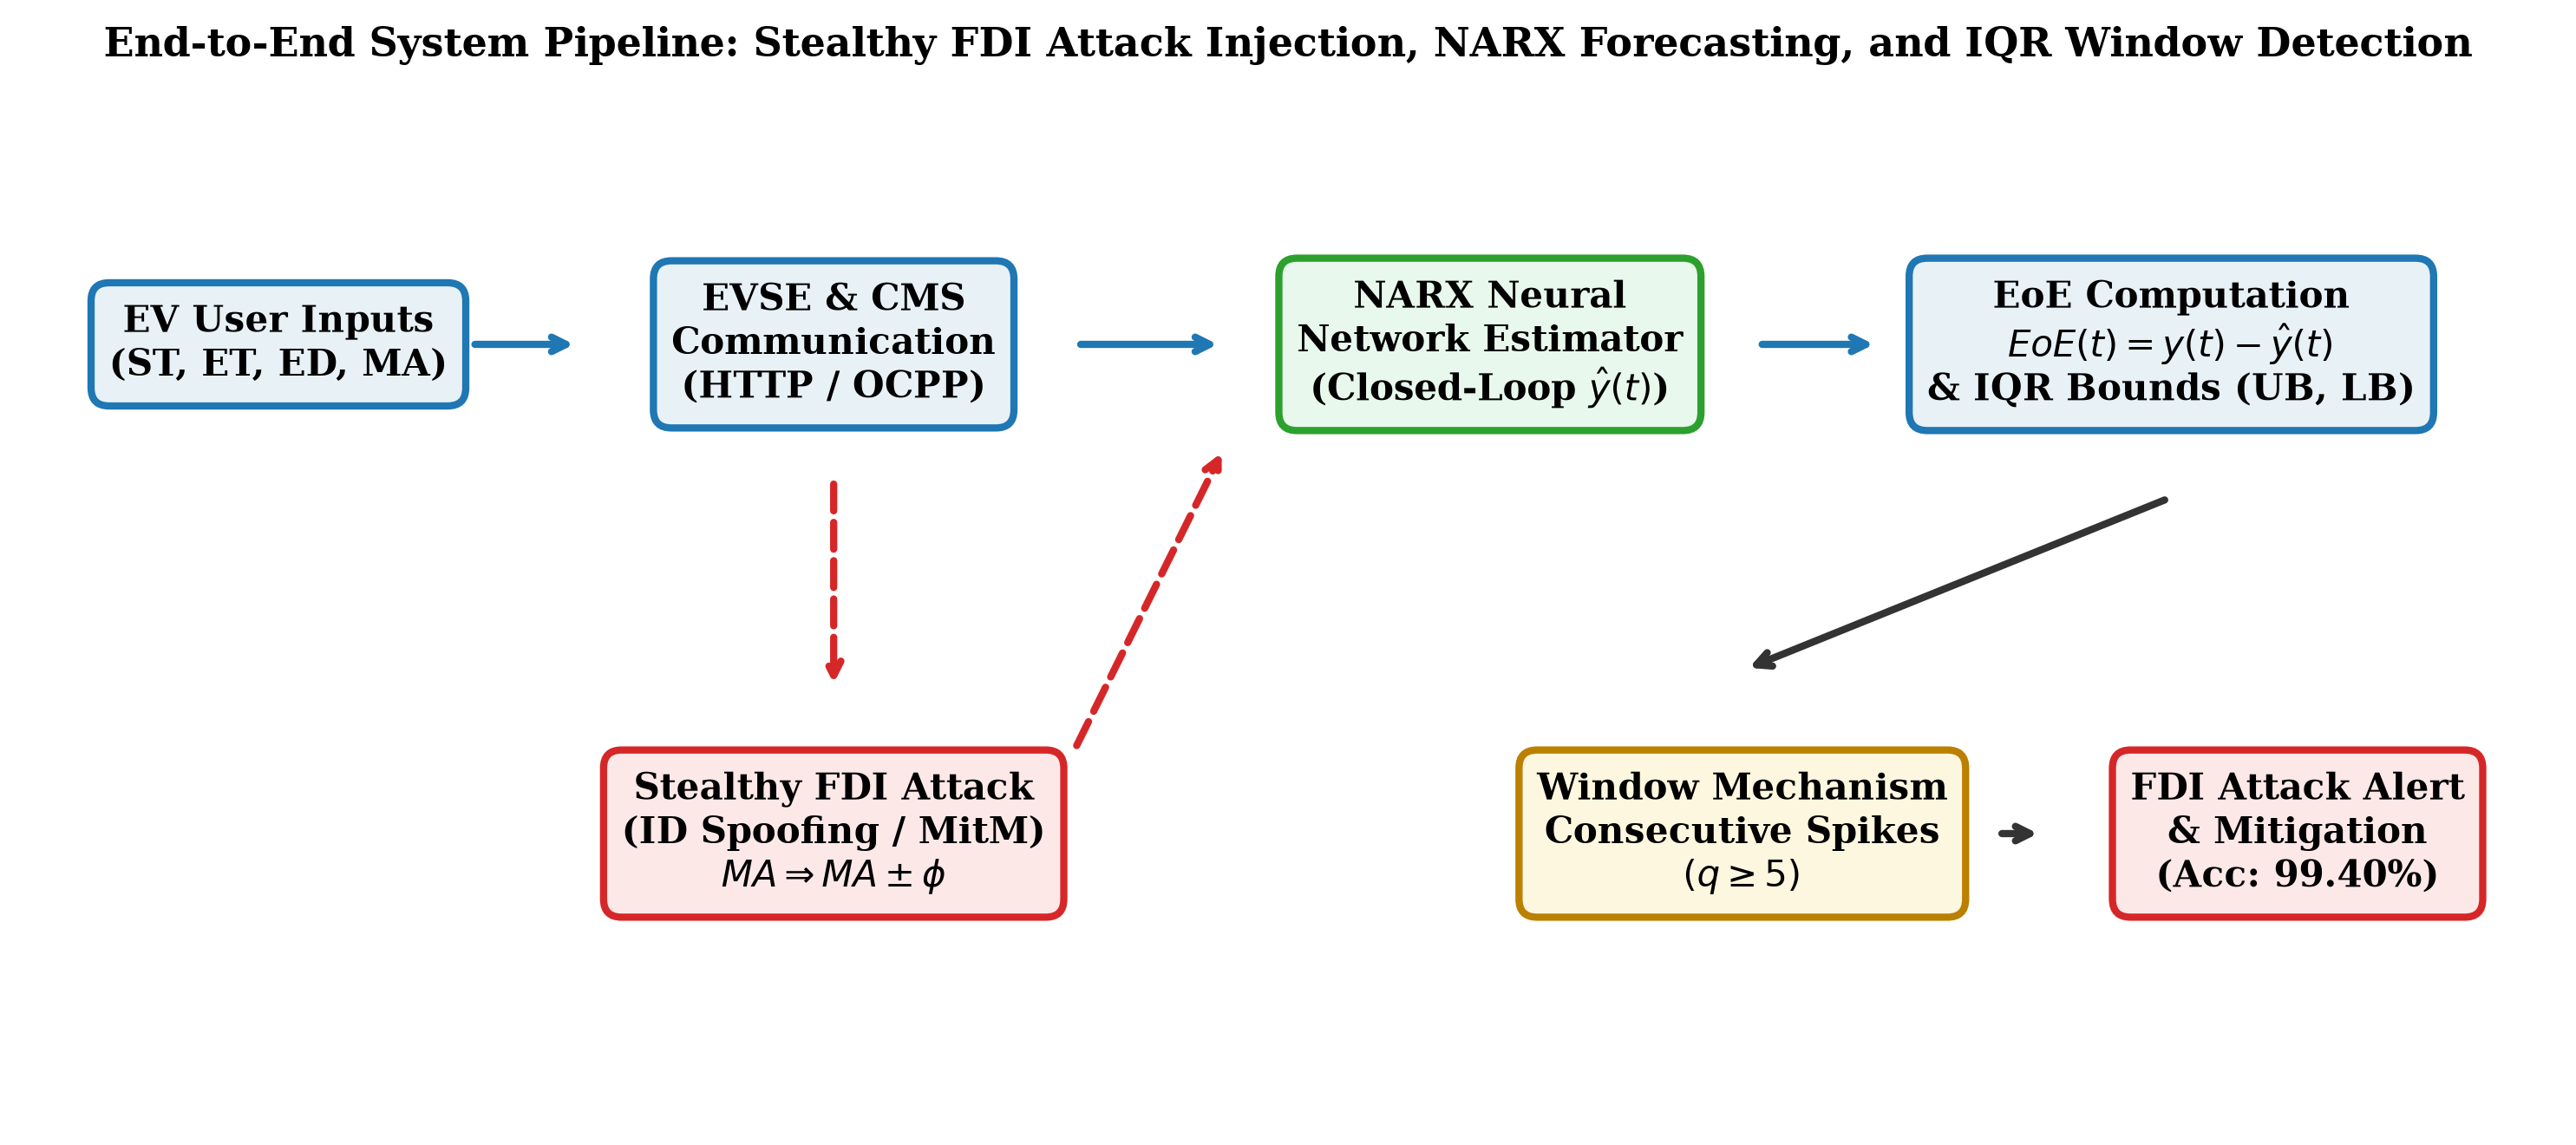
\includegraphics[width=0.92\textwidth]{fig1_flowchart.png}
\caption{End-to-end system flowchart showing EV user parameter injection, communication protocols (HTTP/OCPP), stealthy FDI manipulation, closed-loop NARX energy estimation, EoE computation, IQR statistical bounding, and consecutive spike window alerting.}
\label{fig:pipeline}
\end{figure*}

\section{System Architecture and Threat Model}

\subsection{Communication Protocol Stack and Vulnerabilities}
An IoT-enabled EVCS infrastructure comprises three primary communication layers, each exhibiting distinct vulnerabilities:
\begin{enumerate}
    \item \textbf{User-to-CMS (HTTP/HTTPS)}: EV users submit reservations, requested departure times, and energy demands through mobile applications communicating with the CMS. Session handling over web APIs often remains vulnerable to credential theft, phishing, and identity (ID) spoofing \cite{ElKashlan2023}.
    \item \textbf{EVSE-to-CMS (OCPP)}: The Open Charge Point Protocol coordinates real-time power limits, heartbeat metrics, and transaction status between EVSE units and the central controller \cite{Alcaraz2017}. Insufficient mutual TLS enforcement enables Man-in-the-Middle (MitM) packet manipulation.
    \item \textbf{EVSE-to-BMS (IEC 61851 / ISO 15118)}: Physical charging rate negotiation and battery State-of-Charge (SoC) updates are managed via pilot signals and CAN/PLC links. Tampering with low-level analog pilot signals can forcefully curtail energy flow \cite{Antoun2020}.
\end{enumerate}

\subsection{Stealthy FDI Attack Formulation}
When vehicle $n$ is connected to EVSE $m$ at time $t$, the user specifies four operating parameters: Start Time ($ST_t^n$), End Time ($ET_t^n$), Energy Demanded ($ED_t^n$), and Minutes Available ($MA_t^n$). The CMS calculates an optimal charging session profile $CS_t^n$:
\begin{equation}
CS_t^n = f\left(ST_t^n, ET_t^n, ED_t^n, MA_t^n\right)
\label{eq:session}
\end{equation}

Under benign conditions, users may adjust their available duration at time $t + \Delta t$ to update the schedule. An attacker exploits this valid update mechanism through spoofed HTTP requests or MitM interception by adding a false perturbation $\pm \phi$:
\begin{equation}
MA_{t+\Delta t}^{n, \text{adv}} = MA_t^n - \phi
\label{eq:attack_param}
\end{equation}
\begin{equation}
CS_{t+\Delta t}^{n, \text{adv}} = f\left(ST_t^n, ET_t^n, ED_t^n, MA_{t+\Delta t}^{n, \text{adv}}\right)
\label{eq:attack_session}
\end{equation}

Because scheduling engines prioritize vehicles with shorter availability ($MA$) to maximize station turnover, artificially reducing $MA$ alters the assigned current $I(t)$ and power $P(t) = V(t) \cdot I(t)$. If the attacker specifies an availability that has already lapsed, the EVSE halts charging abruptly. Because the false inputs conform to normal syntax and value ranges, conventional perimeter firewalls cannot detect the anomaly.

\begin{figure*}[!t]
\centering
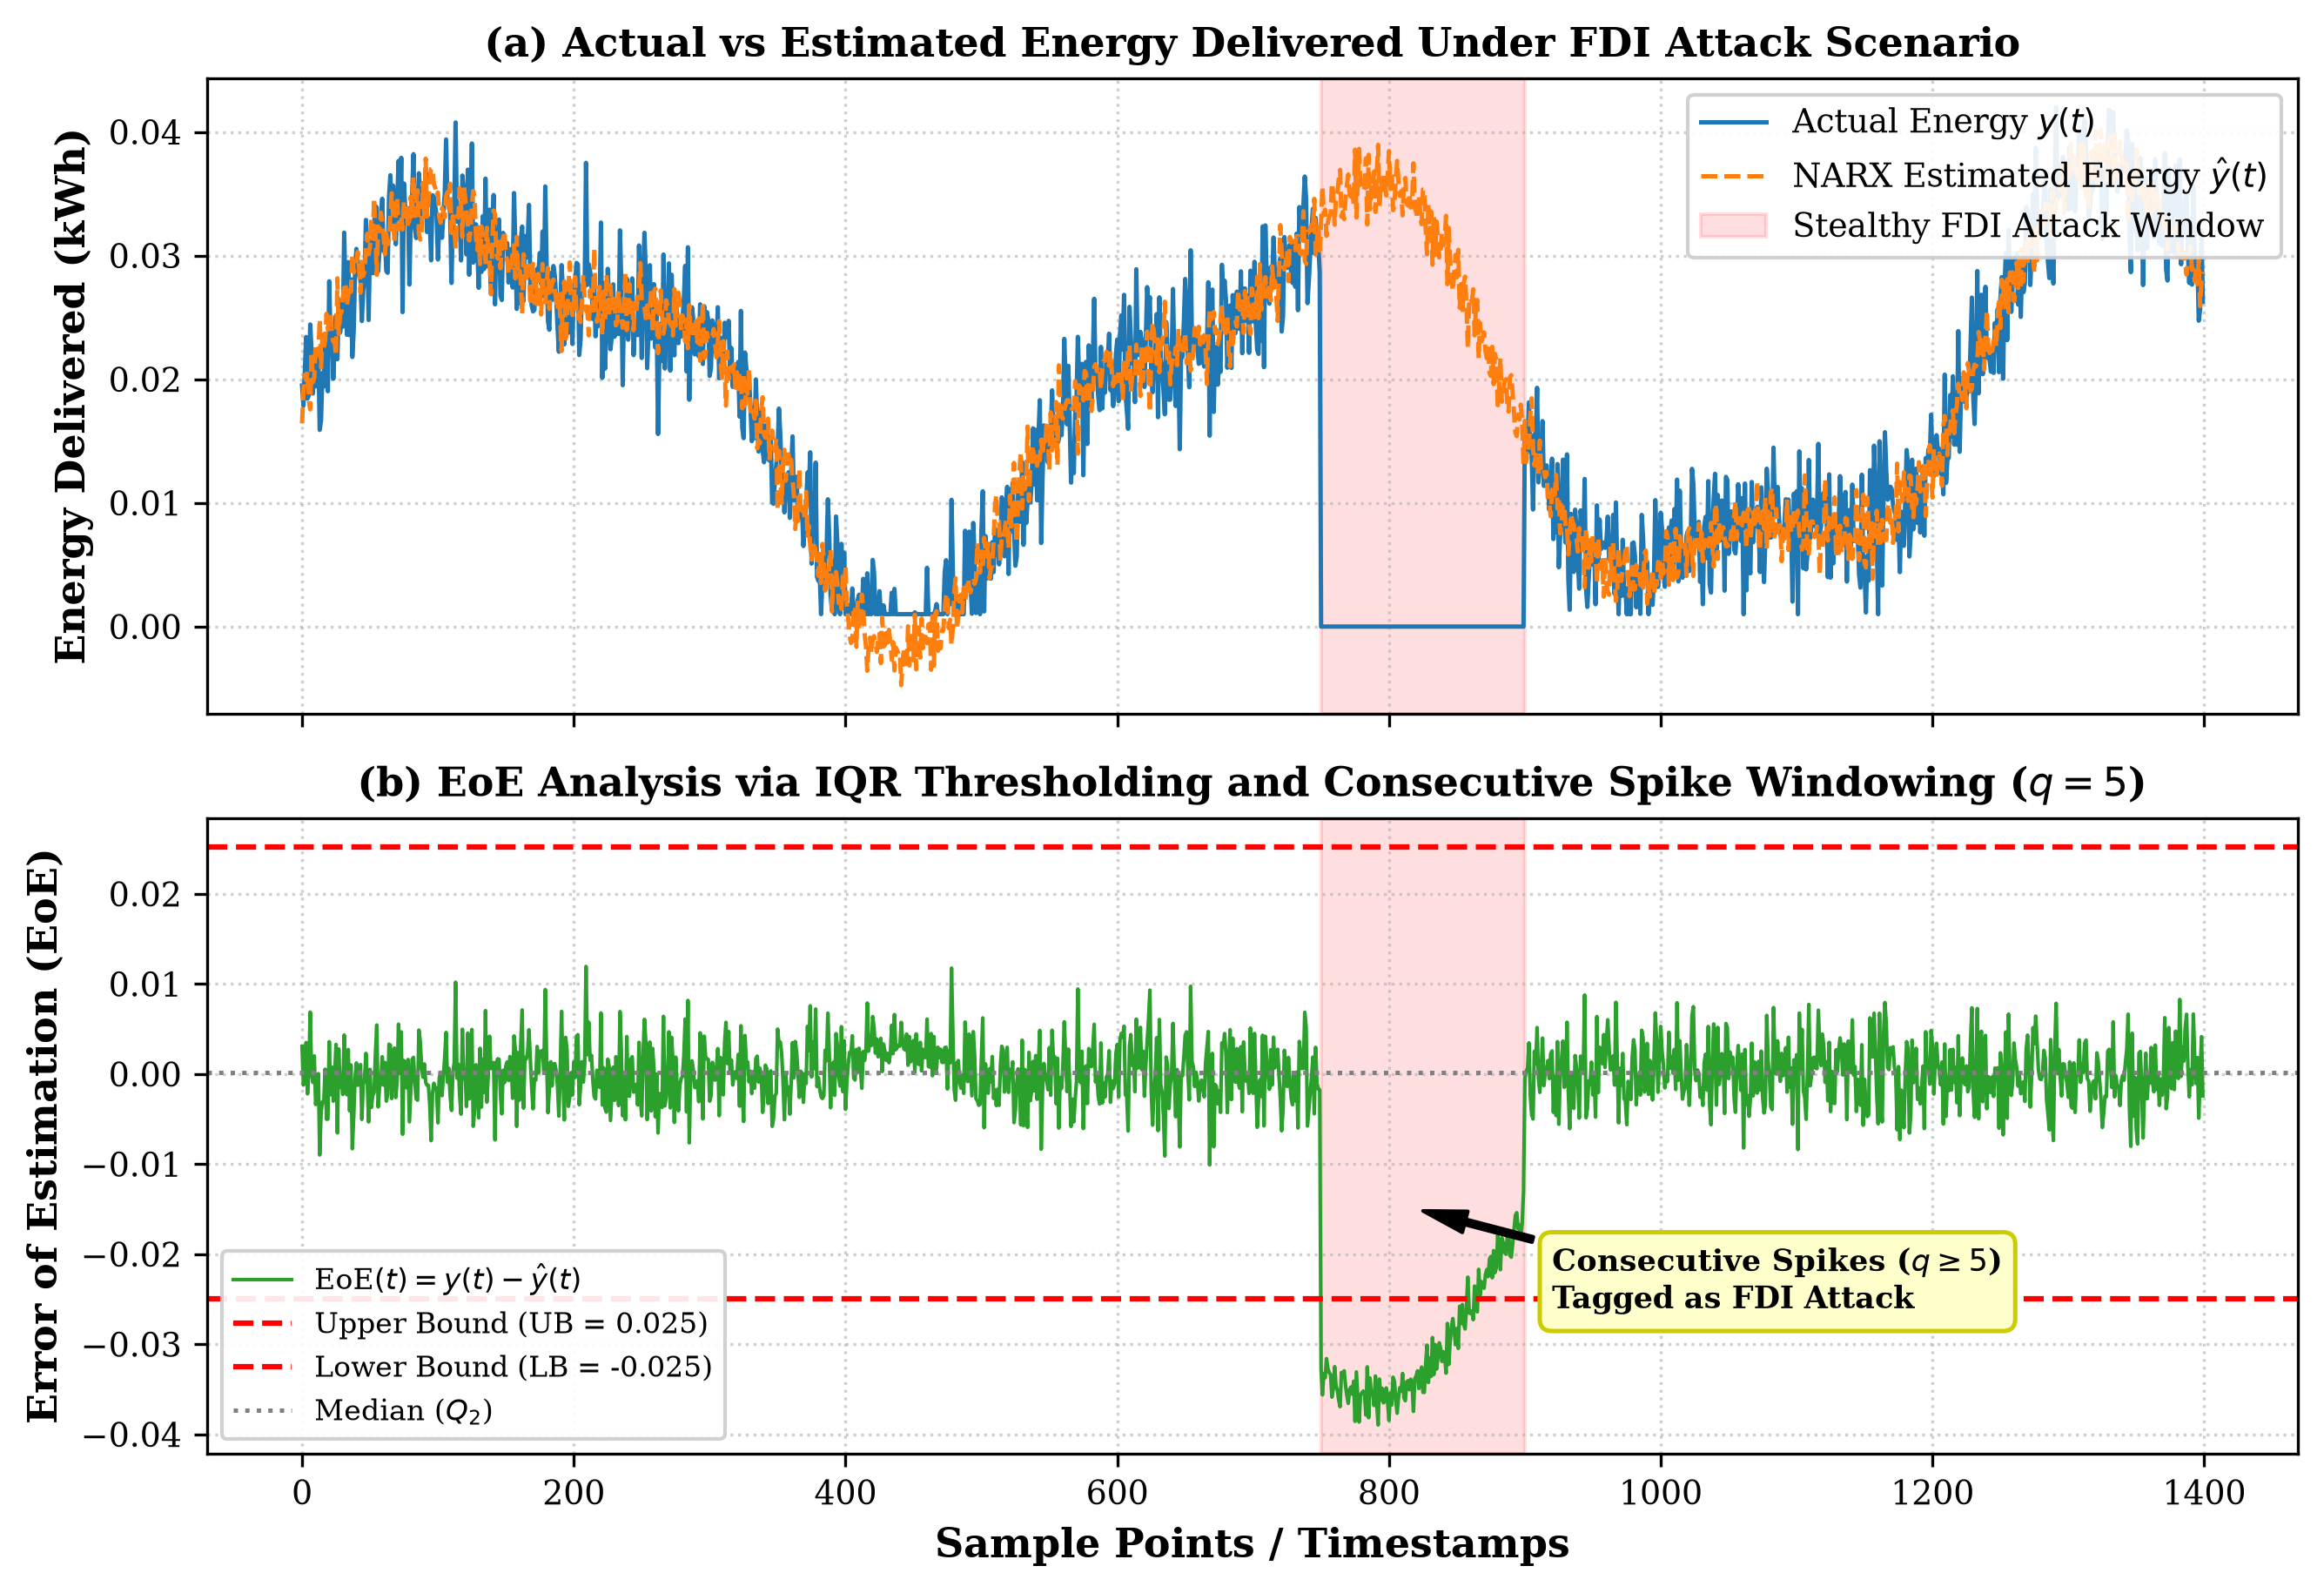
\includegraphics[width=0.92\textwidth]{fig2_attack_iqr.png}
\caption{(a) Actual vs. NARX-estimated energy delivered under a stealthy FDI attack halting charging. (b) EoE time-series with IQR statistical upper/lower bounds and $q=5$ consecutive spike identification flagging the intrusion.}
\label{fig:attack_results}
\end{figure*}

\section{Proposed NARX-IQR Detection Framework}

\subsection{NARX Neural Network Architecture}
The NARX network is a dynamic recurrent neural network with feedback connections across multiple temporal layers \cite{Siegelmann1997}. It maps the continuous dependent output $y(t)$ (energy delivered in kWh per timestamp) using historical values of exogenous inputs $x(t)$ and endogenous feedback $y(t)$:
\begin{equation}
y(t) = F\left(\mathbf{X}(t), \mathbf{Y}(t)\right)
\label{eq:narx_general}
\end{equation}
where:
\begin{align}
\mathbf{X}(t) &= [x(t-1), x(t-2), \dots, x(t-m_x)] \\
\mathbf{Y}(t) &= [y(t-1), y(t-2), \dots, y(t-m_y)]
\end{align}
Here, $m_x$ and $m_y$ denote the memory delay orders for exogenous inputs and endogenous outputs, respectively.

To balance non-linear representation capacity with edge computational efficiency, the proposed network utilizes:
\begin{itemize}
    \item \textbf{Input Layer}: 4 exogenous user parameters ($ST, ET, ED, MA$) plus feedback terms with memory orders $m_x = m_y = 2$.
    \item \textbf{Hidden Layer}: A single hidden layer containing $n_h = 10$ neurons with sigmoid activation functions, trained via the Levenberg-Marquardt algorithm.
    \item \textbf{Output Layer}: A linear node estimating instantaneous delivered energy $\hat{y}(t)$:
\end{itemize}
\begin{equation}
\hat{y}(t) = F_{\text{out}}\left(w_{\text{out}} \cdot F_{\text{hid}}\left(w_{\text{hid}} \mathbf{U}(t-1) + b_{\text{hid}}\right) + b_{\text{out}}\right)
\label{eq:narx_math}
\end{equation}
where $\mathbf{U}(t-1)$ represents the concatenated lagged input-output vector. The model is trained offline in an open-loop configuration and executed online in a closed-loop parallel mode where previous predictions $\hat{y}(t-1)$ are fed back autonomously.

\subsection{Error of Estimation (EoE) Metric}
At each timestamp $t$, the deviation between measured meter energy $y(t)$ and estimated energy $\hat{y}(t)$ is quantified as:
\begin{equation}
EoE(t) = y(t) - \hat{y}(t)
\label{eq:eoe}
\end{equation}
Under uncompromised operation, actual and estimated energy remain tightly synchronized: $EoE(t) \approx 0$. When an FDI attack alters parameters and drops delivered current to zero, the NARX network continues projecting nominal energy based on historical dynamics, causing a large deviation: $|EoE(t)| \gg 0$.

\subsection{IQR Statistical Bounding and Consecutive Spike Windowing}
To avoid arbitrary static thresholds, we establish data-driven bounds via the Interquartile Range (IQR):
\begin{equation}
IQR = Q_3 - Q_1
\label{eq:iqr}
\end{equation}
\begin{equation}
LB = Q_1 - \beta \cdot IQR, \quad UB = Q_3 + \beta \cdot IQR
\label{eq:bounds}
\end{equation}
where $Q_1$ and $Q_3$ denote the 25th and 75th percentiles of the baseline residual distribution, and $\beta = 5.0$ is an empirically determined scale multiplier.

Normal vehicle connection/disconnection transitions and utility grid sags cause isolated single-sample spikes in $EoE(t)$. To prevent false alarms, the framework applies a consecutive spike window filter of size $q = 5$:
\begin{equation}
\text{Alarm}(t) = 
\begin{cases} 
1 \; (\text{Attack}), & \text{if } \sum_{k=0}^{q-1} \mathbb{I}\left(EoE(t-k) \notin [LB, UB]\right) = q \\
0 \; (\text{Normal}), & \text{otherwise}
\end{cases}
\label{eq:window}
\end{equation}
where $\mathbb{I}(\cdot)$ is the indicator function. An attack is declared only if $q$ consecutive samples violate the IQR threshold, effectively filtering out transient benign outliers.

\begin{figure}[!t]
\centering
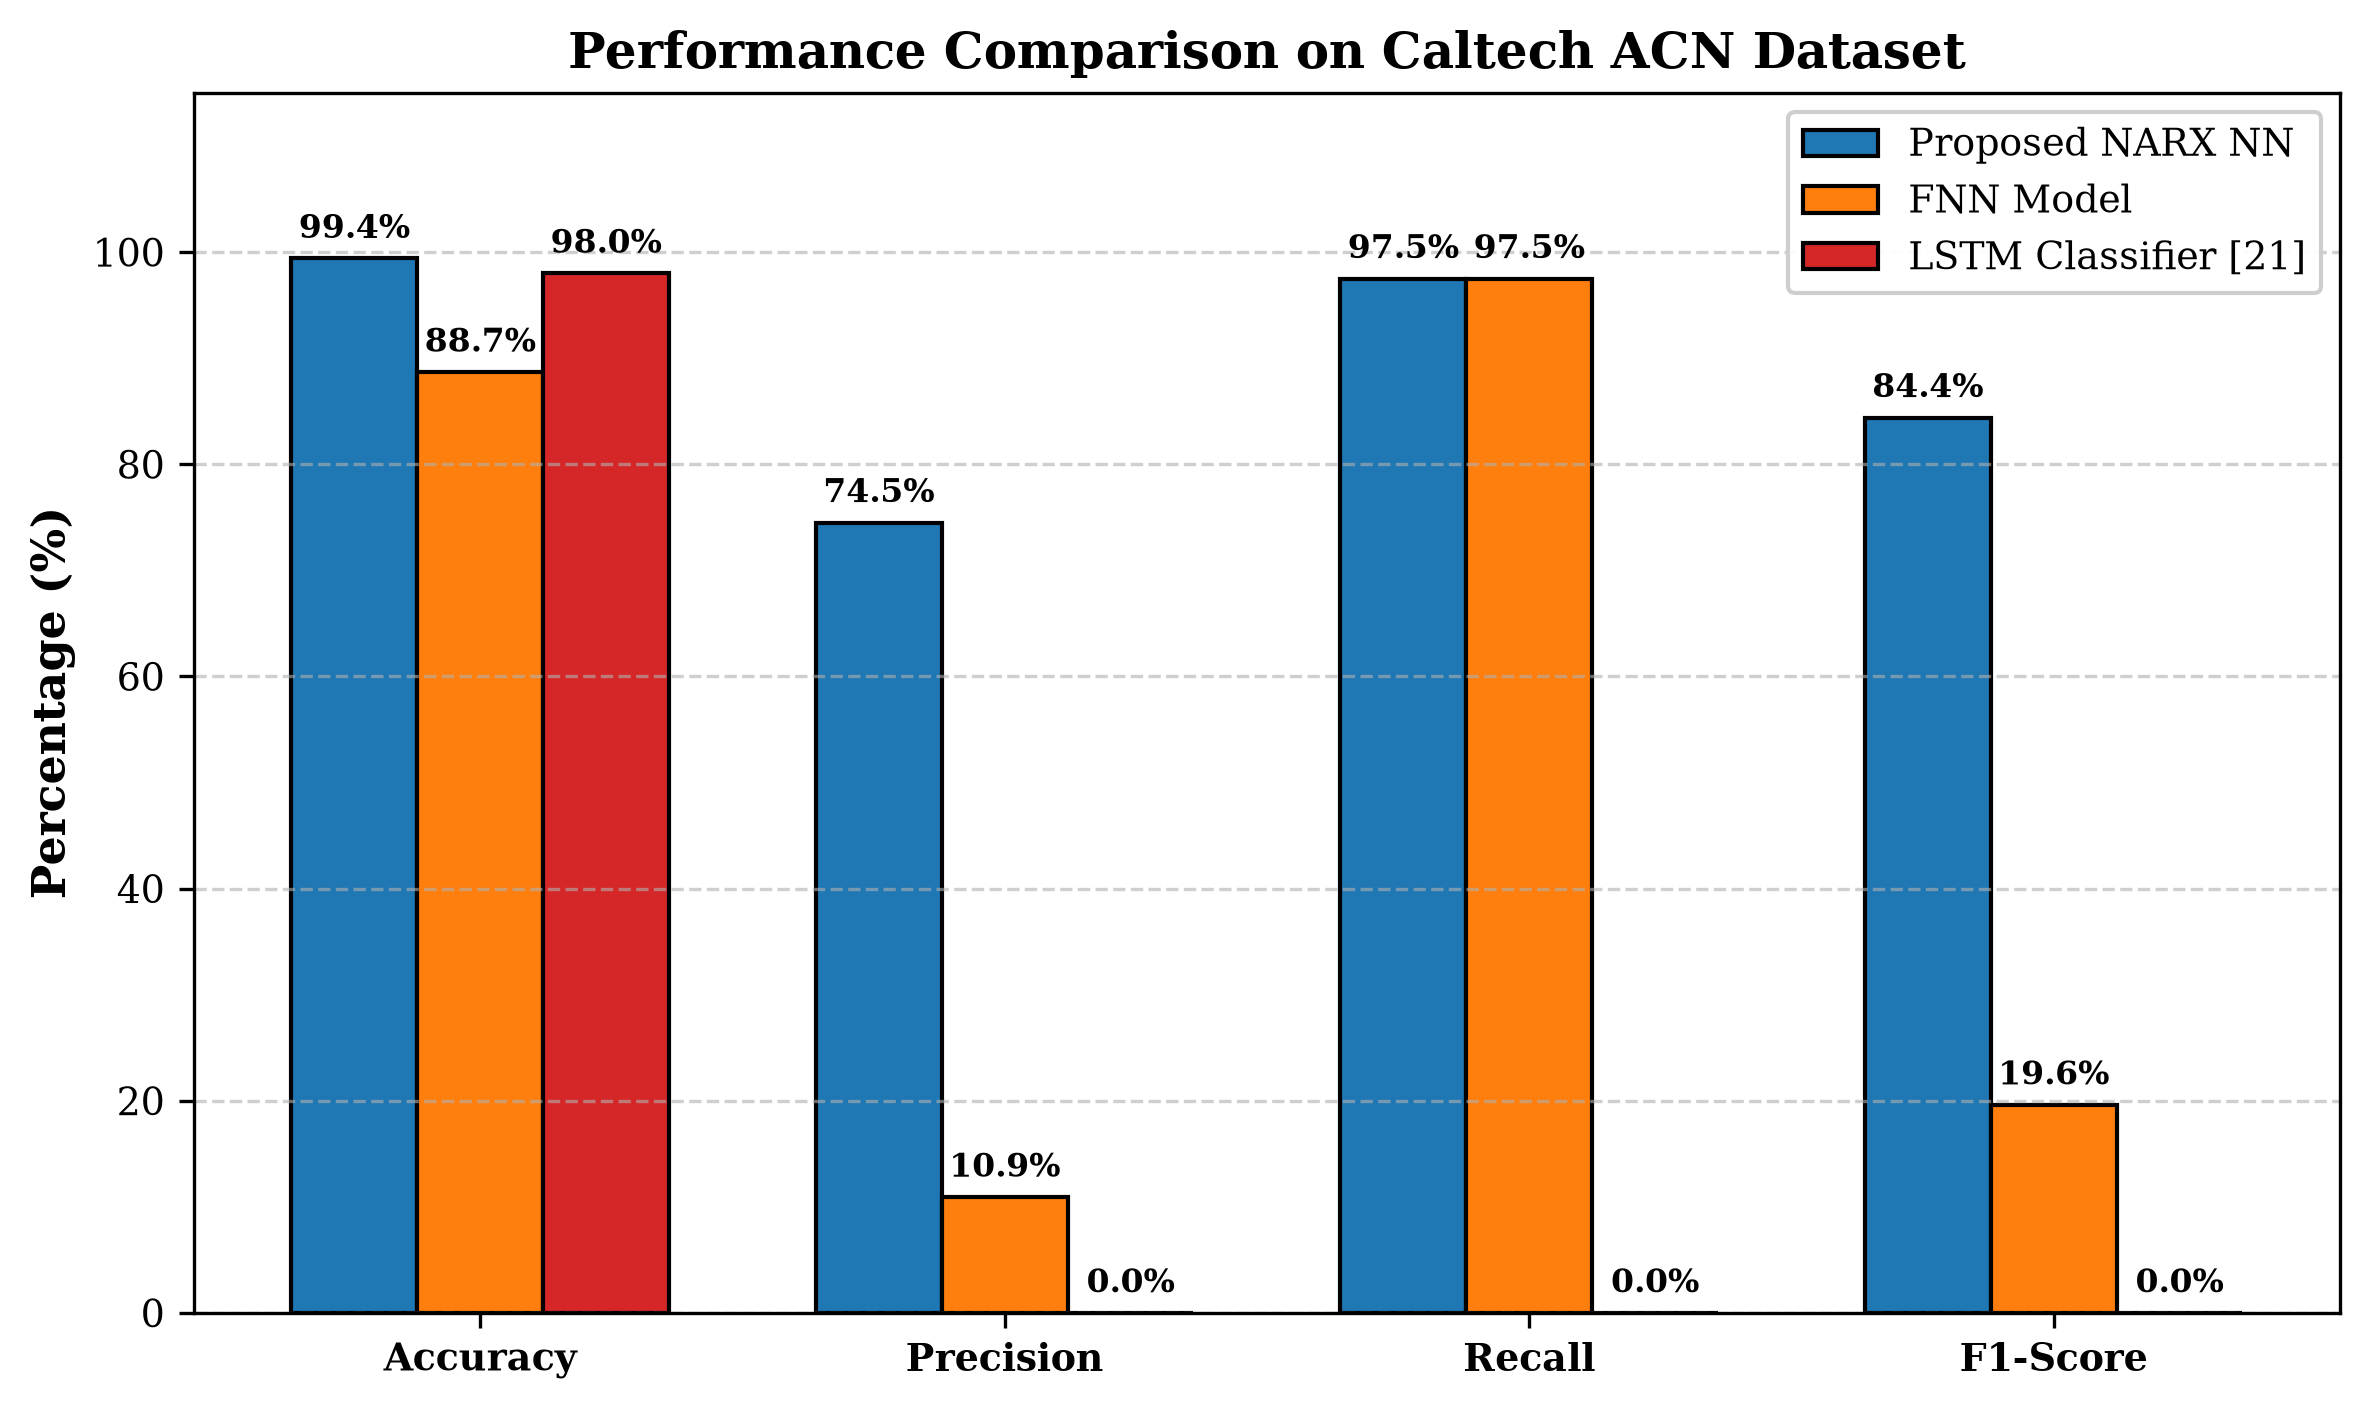
\includegraphics[width=0.48\textwidth]{fig3_comparison.png}
\caption{Performance metric comparison (Accuracy, Precision, Recall, F1-Score) on the Caltech ACN evaluation dataset across the proposed NARX NN, standard FNN, and LSTM binary classifier \cite{Basnet2020}.}
\label{fig:comparison}
\end{figure}

\section{Experimental Setup and Results}

\subsection{Caltech ACN Dataset}
The framework was evaluated using the real-world Caltech Adaptive Charging Network (ACN-Data) benchmark \cite{Lee2019}. The experimental facility comprises 54 EVSEs, an 80-port distribution grid, and a 50-kW DC fast charger. The evaluation dataset spans December 1, 2020 to January 31, 2021 (37.2 MB raw data). After removing incomplete records and non-charging idle intervals, 47,095 clean samples across 169 charging sessions (27 users, 19 EVSEs) were retained. 
\begin{itemize}
    \item \textbf{Training Set}: 32,966 samples (70\% train, 15\% validation, 15\% test).
    \item \textbf{Evaluation Set}: 14,129 unseen samples under normal and injected FDI attack scenarios.
\end{itemize}

\subsection{Detection Performance Comparison}
The proposed NARX framework is benchmarked against:
\begin{enumerate}
    \item An identical-dimension Feedforward Neural Network (FNN) regression model (10 neurons, sigmoid activation) paired with IQR thresholding.
    \item An LSTM binary classifier structured according to recent EVCS intrusion detection literature \cite{Basnet2020}.
\end{enumerate}

Standard evaluation metrics are computed:
\begin{equation}
\text{Precision} = \frac{TP}{TP + FP}, \quad \text{Recall} = \frac{TP}{TP + FN}
\end{equation}
\begin{equation}
F_1\text{-score} = 2 \cdot \frac{\text{Precision} \cdot \text{Recall}}{\text{Precision} + \text{Recall}}
\end{equation}

\begin{table}[!t]
\caption{Quantitative Performance Comparison on ACN Dataset}
\label{tab:comparison}
\centering
\begin{tabular}{lccc}
\toprule
\textbf{Performance Metric} & \textbf{Proposed NARX} & \textbf{FNN Model} & \textbf{LSTM Classifier \cite{Basnet2020}} \\
\midrule
Accuracy (\%)       & \textbf{99.40\%} & 88.68\% & 98.00\% \\
Precision (\%)      & \textbf{74.50\%} & 10.90\% & 0.00\% \\
Recall (\%)         & \textbf{97.50\%} & \textbf{97.50\%} & 0.00\% \\
F1-Score (\%)       & \textbf{84.40\%} & 19.60\% & 0.00\% \\
Mean Squared Error  & \textbf{$1.997 \times 10^{-5}$} & $1.179 \times 10^{-4}$ & N/A \\
\bottomrule
\end{tabular}
\end{table}

\begin{table}[!t]
\caption{Confusion Matrix for the Proposed NARX-IQR Scheme}
\label{tab:conf_narx}
\centering
\begin{tabular}{lcc}
\toprule
& \textbf{Predicted Normal} & \textbf{Predicted Attack} \\
\midrule
\textbf{Actual Normal} & $TN = 13,861$ & $FP = 67$ \\
\textbf{Actual Attack} & $FN = 5$ & $TP = 196$ \\
\bottomrule
\end{tabular}
\end{table}

\begin{table}[!t]
\caption{Confusion Matrix for the FNN Regression Model}
\label{tab:conf_fnn}
\centering
\begin{tabular}{lcc}
\toprule
& \textbf{Predicted Normal} & \textbf{Predicted Attack} \\
\midrule
\textbf{Actual Normal} & $TN = 12,335$ & $FP = 1,593$ \\
\textbf{Actual Attack} & $FN = 5$ & $TP = 196$ \\
\bottomrule
\end{tabular}
\end{table}

\subsection{Discussion of Findings}
As summarized in Table~\ref{tab:comparison} and illustrated in Fig.~\ref{fig:comparison}:
\begin{itemize}
    \item \textbf{NARX vs. FNN}: The recurrent delay memory embedded in NARX enables it to capture non-linear temporal energy trends far better than FNN, yielding an order-of-magnitude lower MSE ($1.997 \times 10^{-5}$ vs. $1.179 \times 10^{-4}$). Consequently, FNN generates 1,593 false positives compared to just 67 for NARX, resulting in a low FNN precision of 10.90\%.
    \item \textbf{Failure of Classifier Baselines (LSTM)}: In real-world charging traces, attack samples constitute less than 1.5\% of data points. When trained on this imbalanced dataset, the LSTM classifier achieves 98.00\% raw accuracy solely by classifying all instances as non-attack ($TN = 13,928, FN = 201, TP = 0$). It yields 0\% precision and 0\% recall. In contrast, the proposed NARX regression framework optimizes continuous squared errors across all time steps, remaining completely robust to class label imbalance.
\end{itemize}

\begin{figure}[!t]
\centering
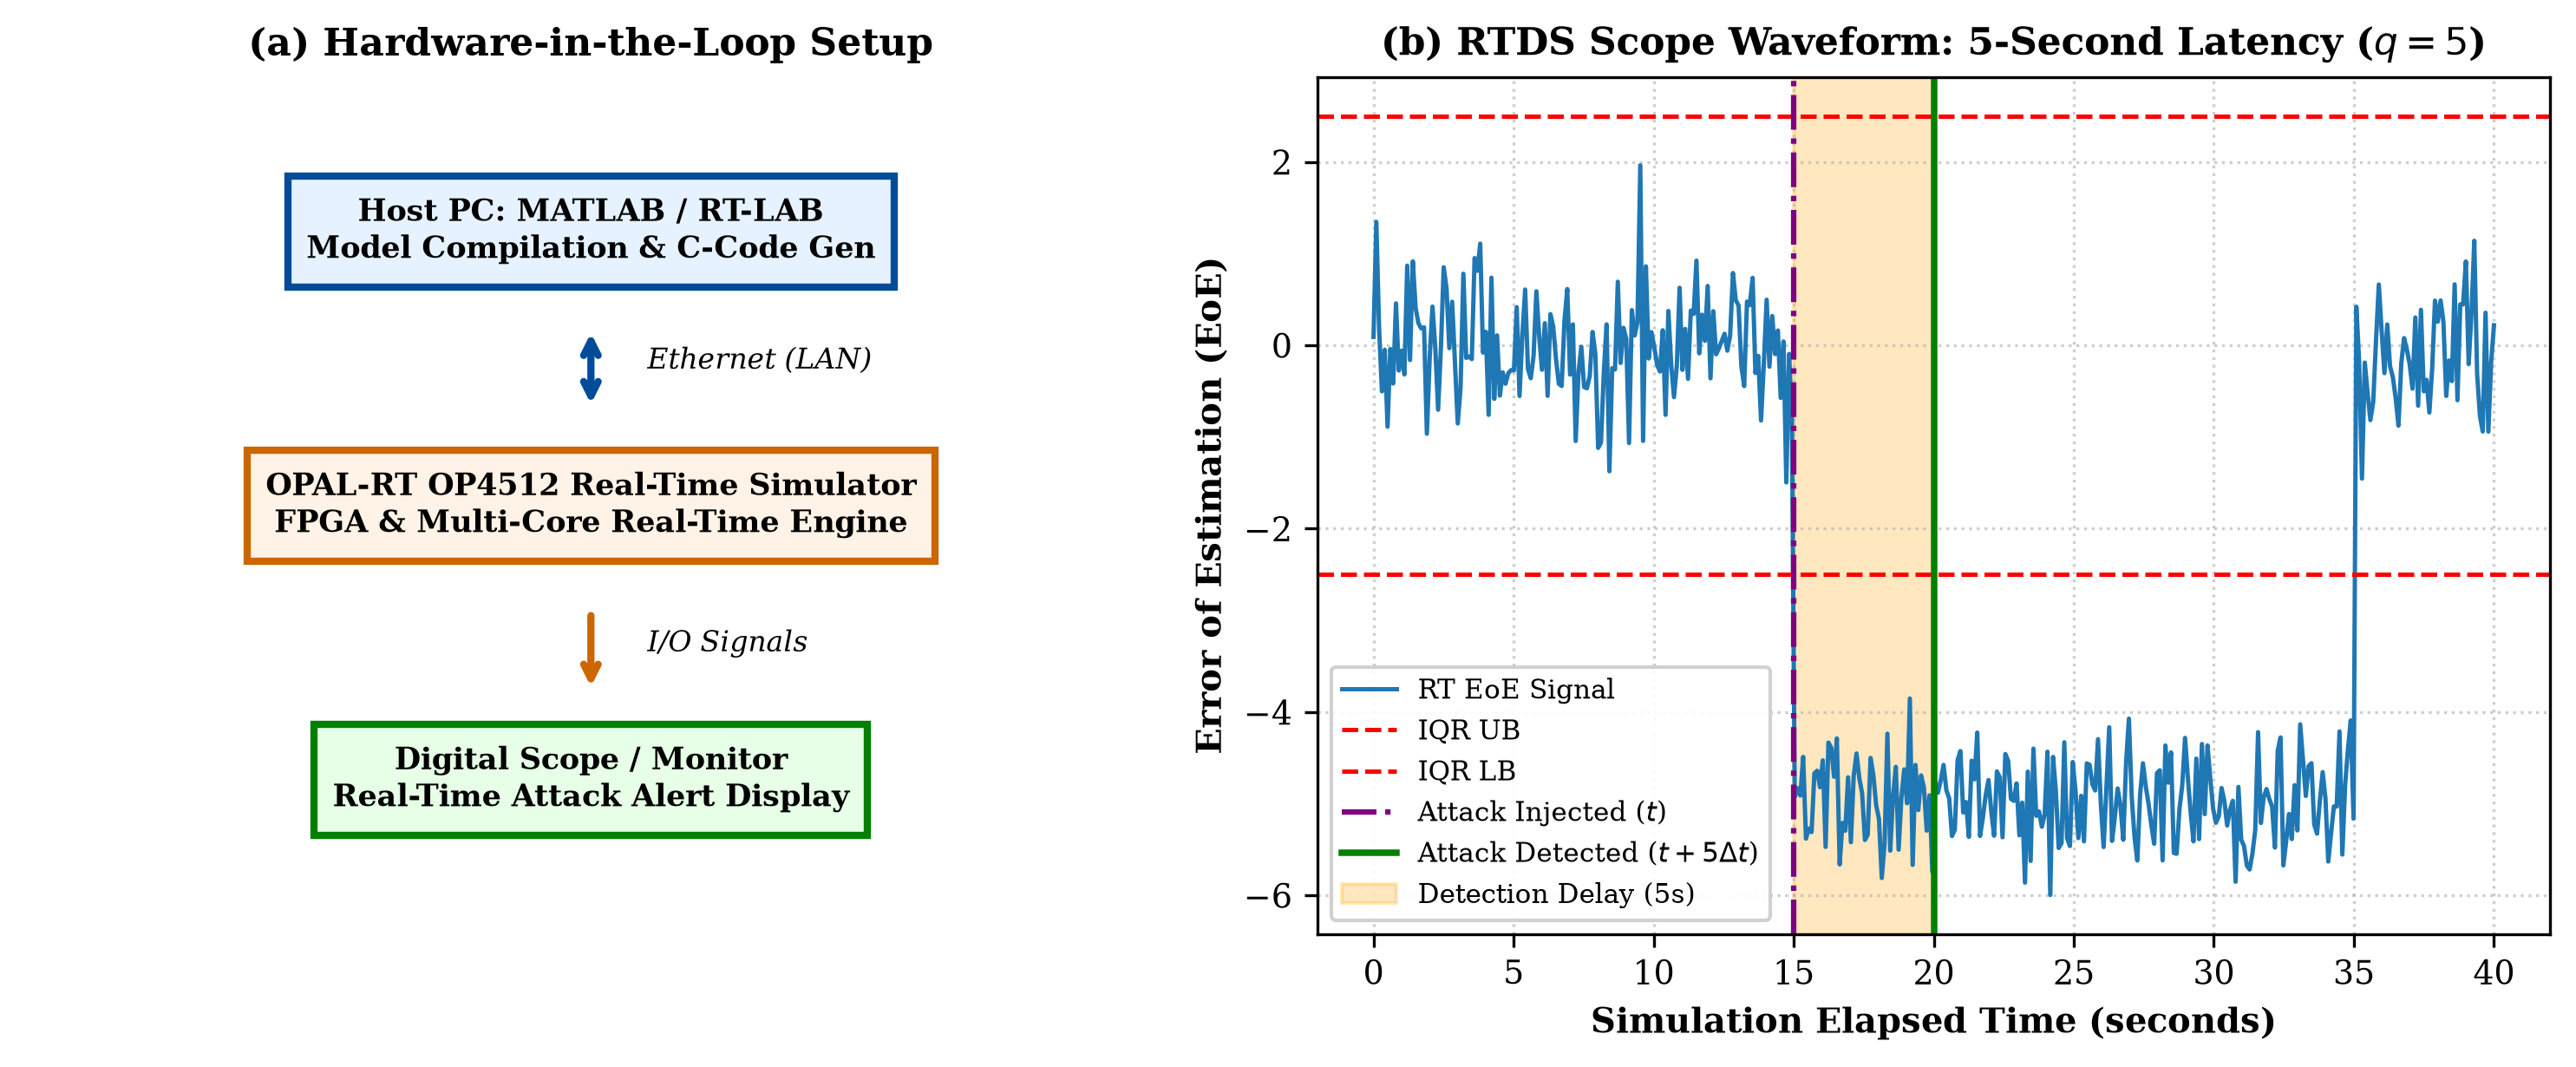
\includegraphics[width=0.48\textwidth]{fig4_opal_rt.png}
\caption{(a) OPAL-RT OP4512 hardware-in-the-loop simulation environment. (b) RTDS scope waveform showing injection at sample 8,000 (2h 13m 20s) and detection at sample 8,005 (2h 13m 25s) with exactly 5-second latency ($q=5$).}
\label{fig:hardware}
\end{figure}

\section{Real-Time Hardware Validation on OPAL-RT}
To validate real-time operational feasibility on embedded microgrid controllers, the framework was executed on an OPAL-RT OP4512 Real-Time Digital Simulator (RTDS) integrated with RT-LAB and MATLAB/Simulink (Fig.~\ref{fig:hardware}(a)).

The 14,129 evaluation samples were streamed at a rate of 1 sample per second. An FDI attack was injected at sample point 8,000 (elapsed simulation time: 2 hours, 13 minutes, 20 seconds). The hardware controller triggered the FDI alarm at sample point 8,005 (2 hours, 13 minutes, 25 seconds). The observed detection latency was **exactly 5 seconds**, directly matching the window length $q = 5$ time steps (Fig.~\ref{fig:hardware}(b)). This confirms that the lightweight NARX model executes within standard real-time control intervals without computational drift.

\section{Limitations and Proposed Project Extensions}
While the proposed framework achieves high detection accuracy and low latency, several open challenges remain:
\begin{enumerate}
    \item \textbf{Short-Duration Attacks}: Attacks persisting for fewer than $q = 5$ time steps evade the window counter.
    \item \textbf{Subtle Injections}: Very minor parameter perturbations produce residuals that remain within the $[LB, UB]$ margin.
    \item \textbf{Static Heuristics}: The multiplier $\beta = 5$ and window size $q = 5$ are fixed and cannot adapt to grid volatility.
\end{enumerate}

\subsection{Proposed Technical Extensions for Upcoming Reviews}
To address these limitations in subsequent project reviews, our team proposes the following technical contributions:
\begin{itemize}
    \item \textbf{Adaptive Dynamic IQR \& Windowing}: We will develop an online Bayesian tuning scheme that continuously adjusts $\beta(t)$ and $q(t)$ based on rolling grid variance, improving detection of short-burst attacks.
    \item \textbf{Attention-Augmented NARX (NARX-Transformer)}: We will integrate a lightweight multi-head self-attention layer to capture cross-station dependencies across neighboring EVSE units.
    \item \textbf{Multi-Parameter Attack Resiliency}: We will expand the framework to defend against simultaneous manipulation of Energy Demanded ($ED$), Start Time ($ST$), and dynamic pricing tariff streams.
    \item \textbf{Edge AI Quantization}: We will quantize the model to 8-bit integer (INT8) representation for direct deployment on low-cost ARM Cortex-M microcontrollers embedded inside commercial Level 2 EVSEs.
\end{itemize}

\section{Conclusion}
This report presented a robust, model-free regression framework using a NARX neural network to detect stealthy False Data Injection attacks in IoT-connected EV charging networks. By forecasting delivered energy and applying Interquartile Range thresholding with a 5-step consecutive spike window, the model avoids false alarms from normal session transitions while circumventing the severe class-imbalance failures of traditional ML classifiers. Tested on 47,095 real-world Caltech ACN samples, the framework achieved 99.40\% accuracy, 74.50\% precision, and an 84.40\% F1-score. Hardware validation on an OPAL-RT simulator confirmed reliable detection within 5 seconds. The identified limitations will guide our upcoming work on adaptive thresholding and multi-parameter cyber-resilience.

\bibliographystyle{IEEEtran}
\bibliography{references}

\end{document}
